

\section{Results}\label{sec:results}

\begin{figure*}[ht]
  \centering
  \resizebox{\hsize}{!}{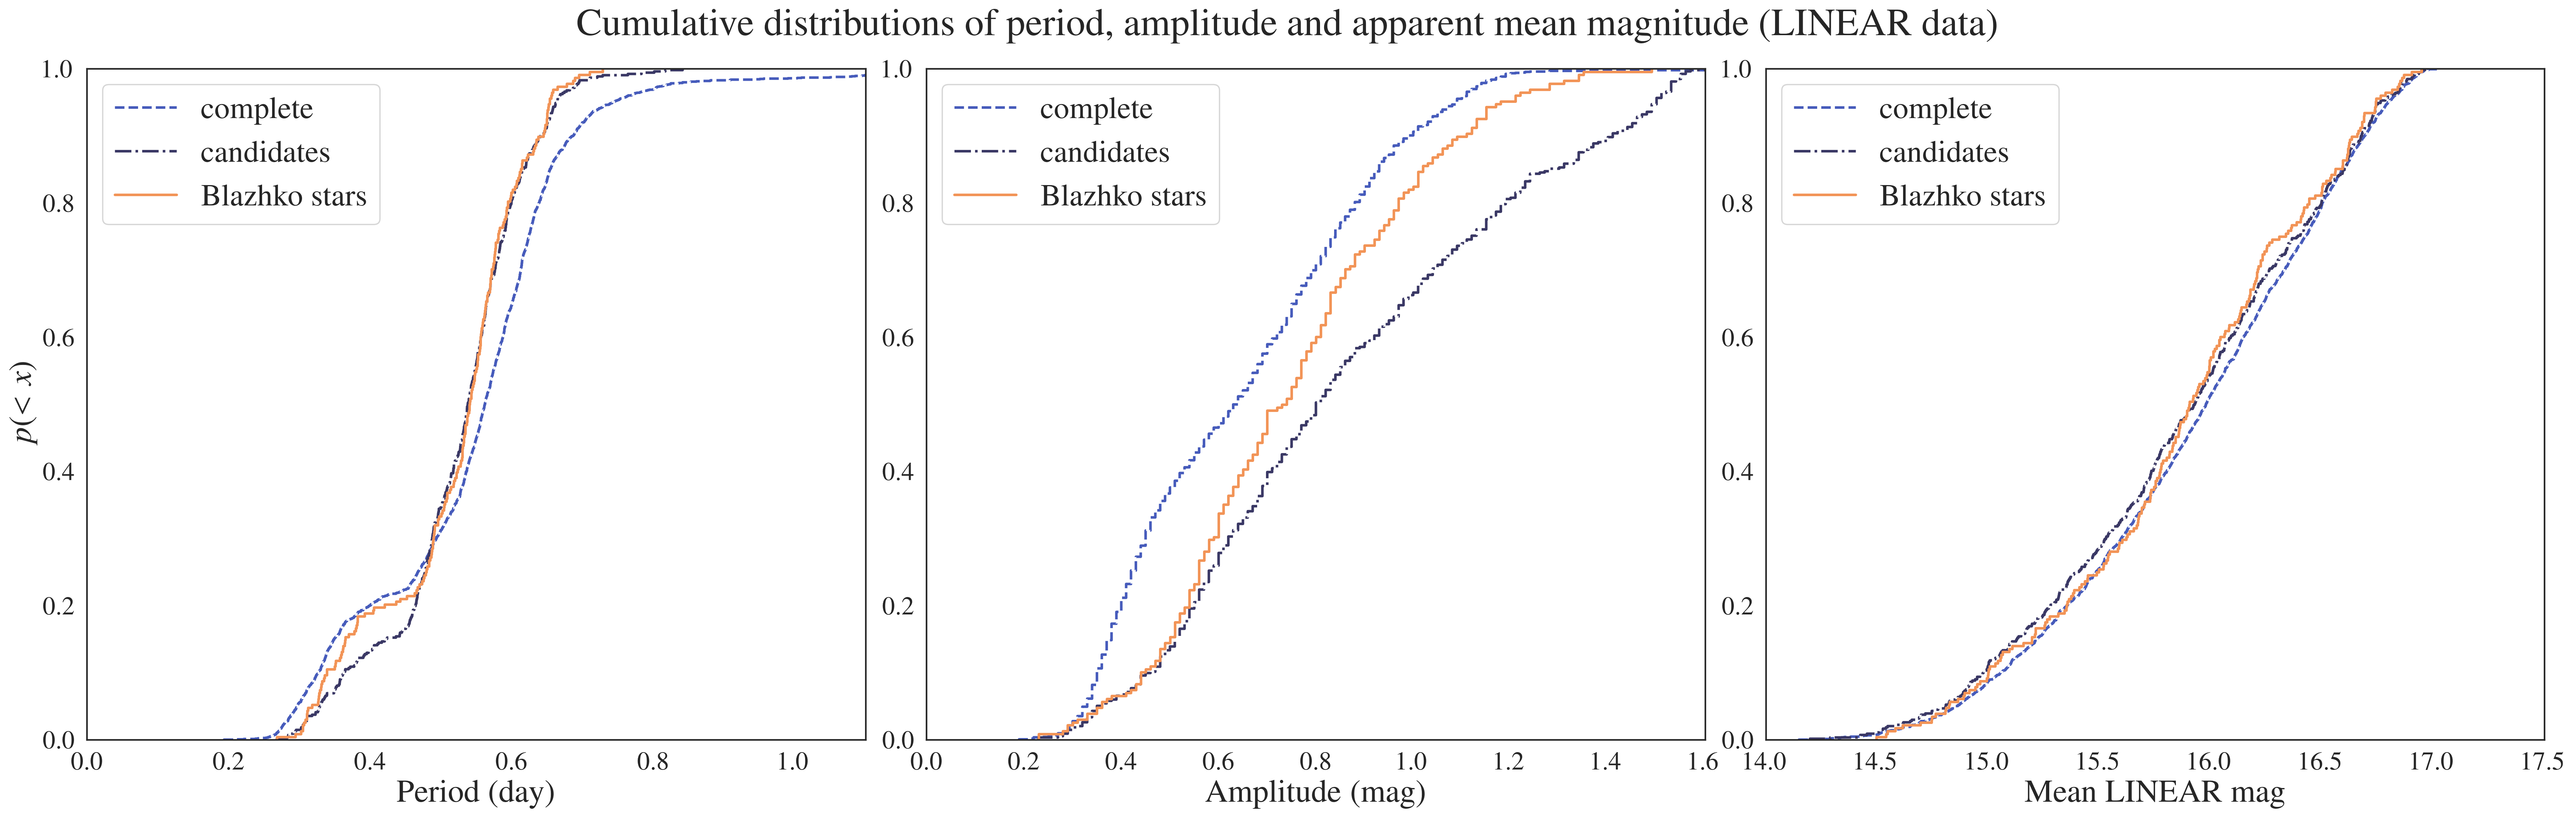
\includegraphics[width=16cm]{cumulative_distib_L.png}}
   \resizebox{\hsize}{!}{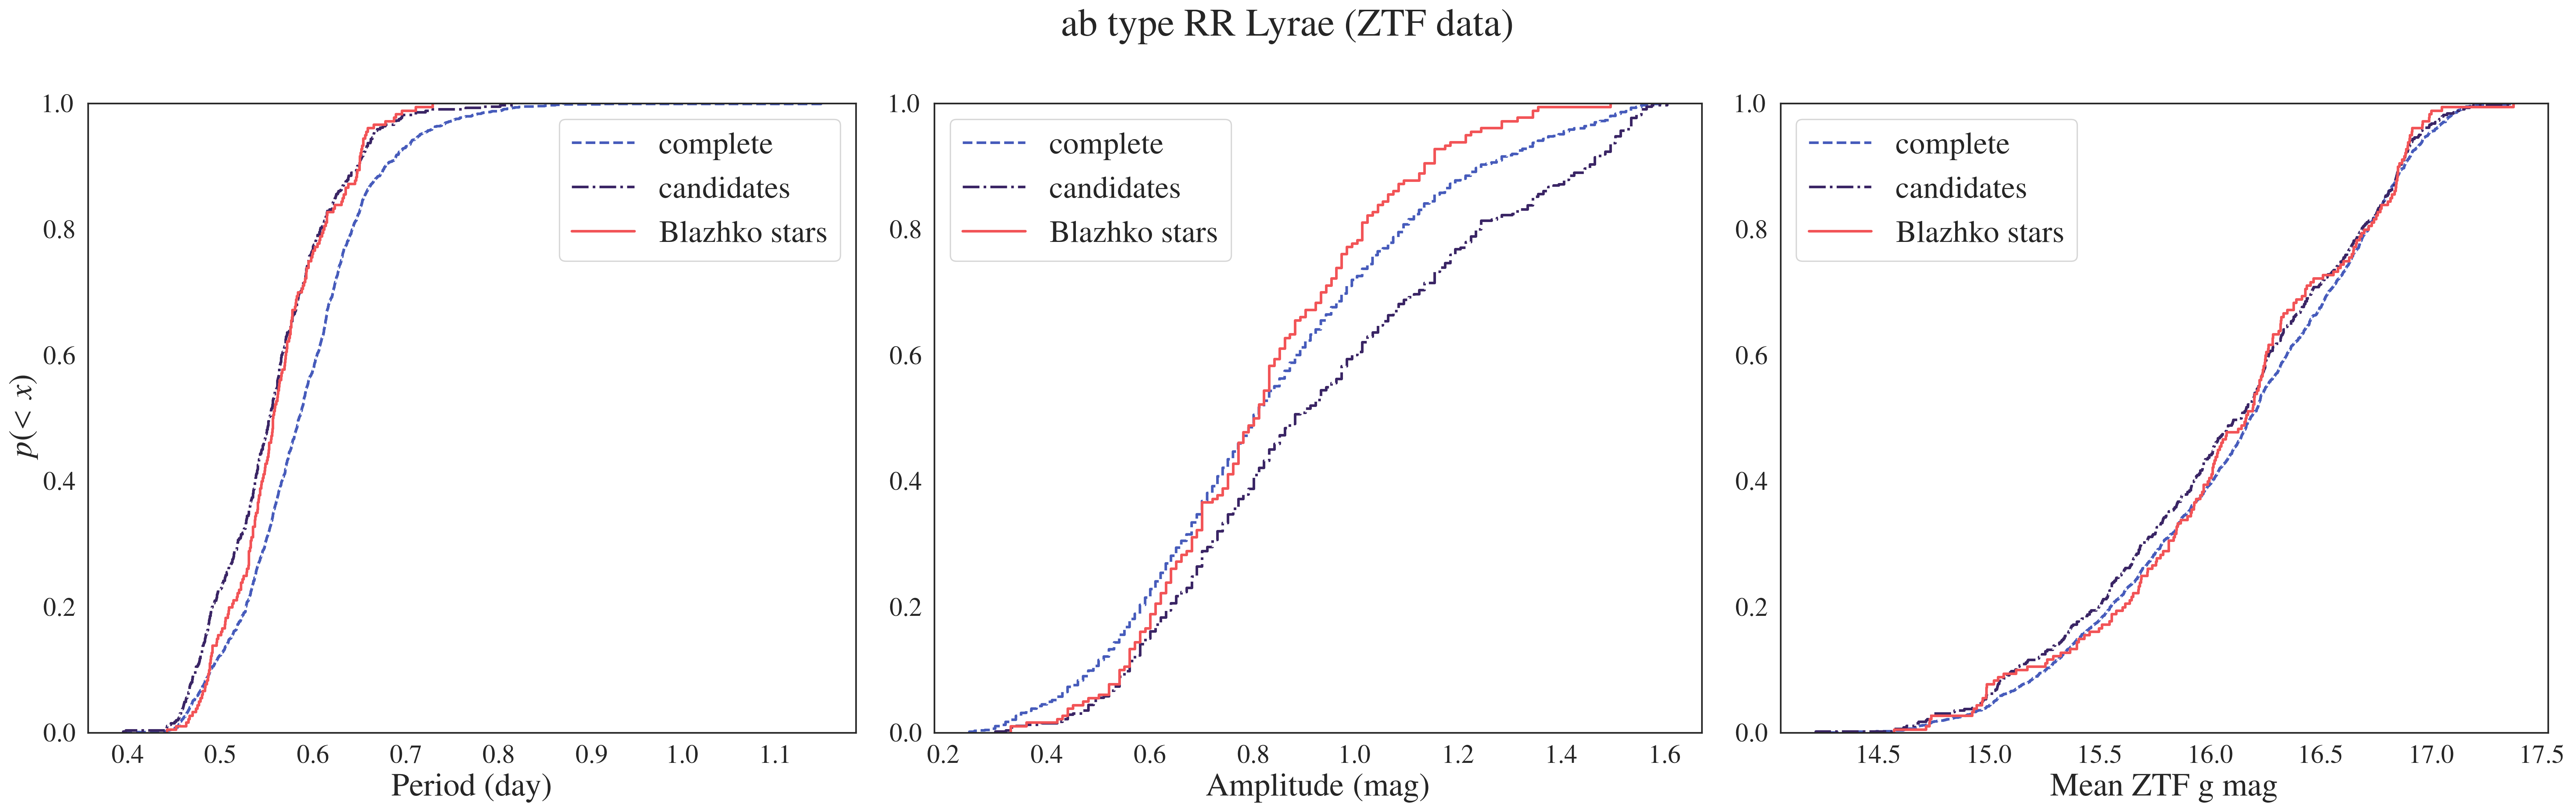
\includegraphics[width=16cm]{CDF_abtype.png}}
   \resizebox{\hsize}{!}{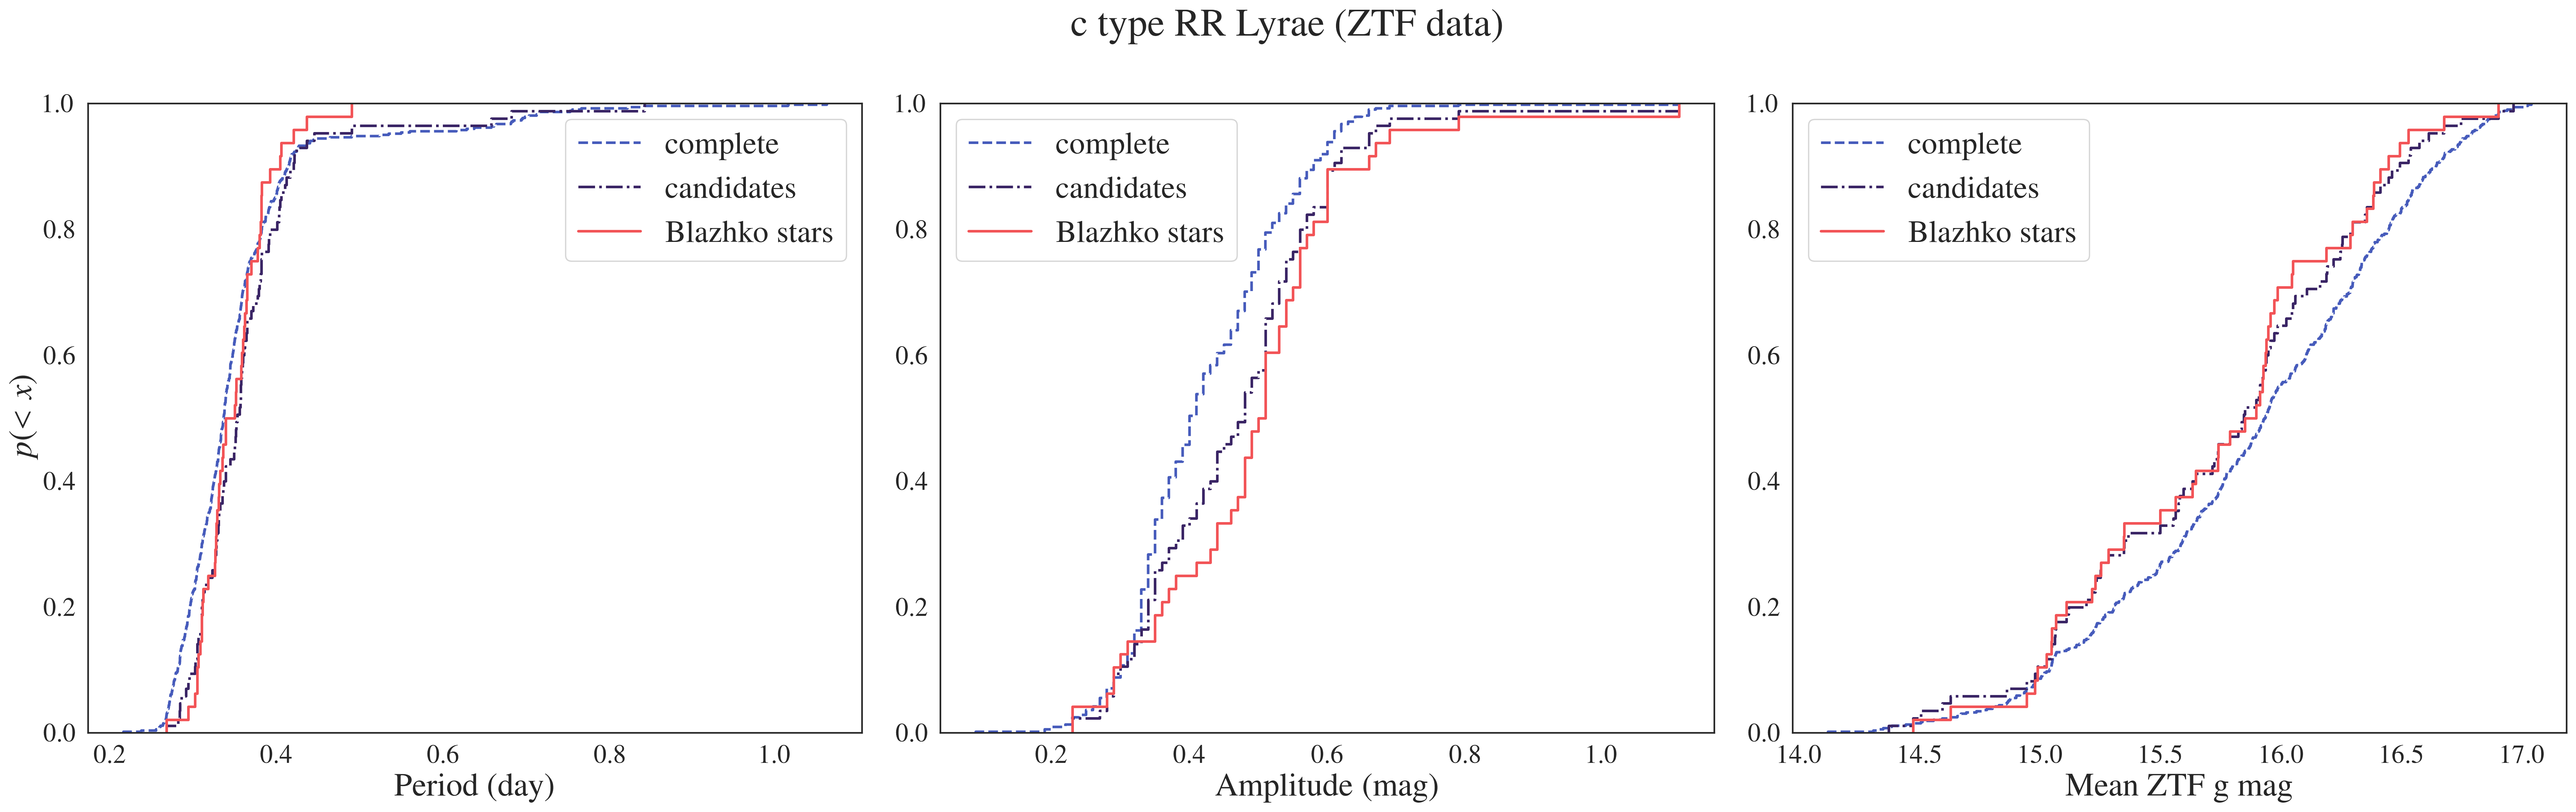
\includegraphics[width=16cm]{CDF_ctype.png}}
 \caption{A comparison of cumulative distributions of period (left),
 amplitude (middle) and apparent magnitude for starting sample,
 selected Blazhko candidates and visually verified Blazhko
 stars. The top row is based on LINEAR data and both ab type and c
 type stars. The middle and bottom rows are
 based on ZTF data, and show separately data for ab type and c type
 stars, respectively. The differences in period and amplitude
 distributions are futher examined in figure~\ref{fig:AmplPeriod2D}.}
    \label{fig:AmplPeriod}
\end{figure*}


\begin{figure*}[ht]
  \centering
  \resizebox{\hsize}{!}{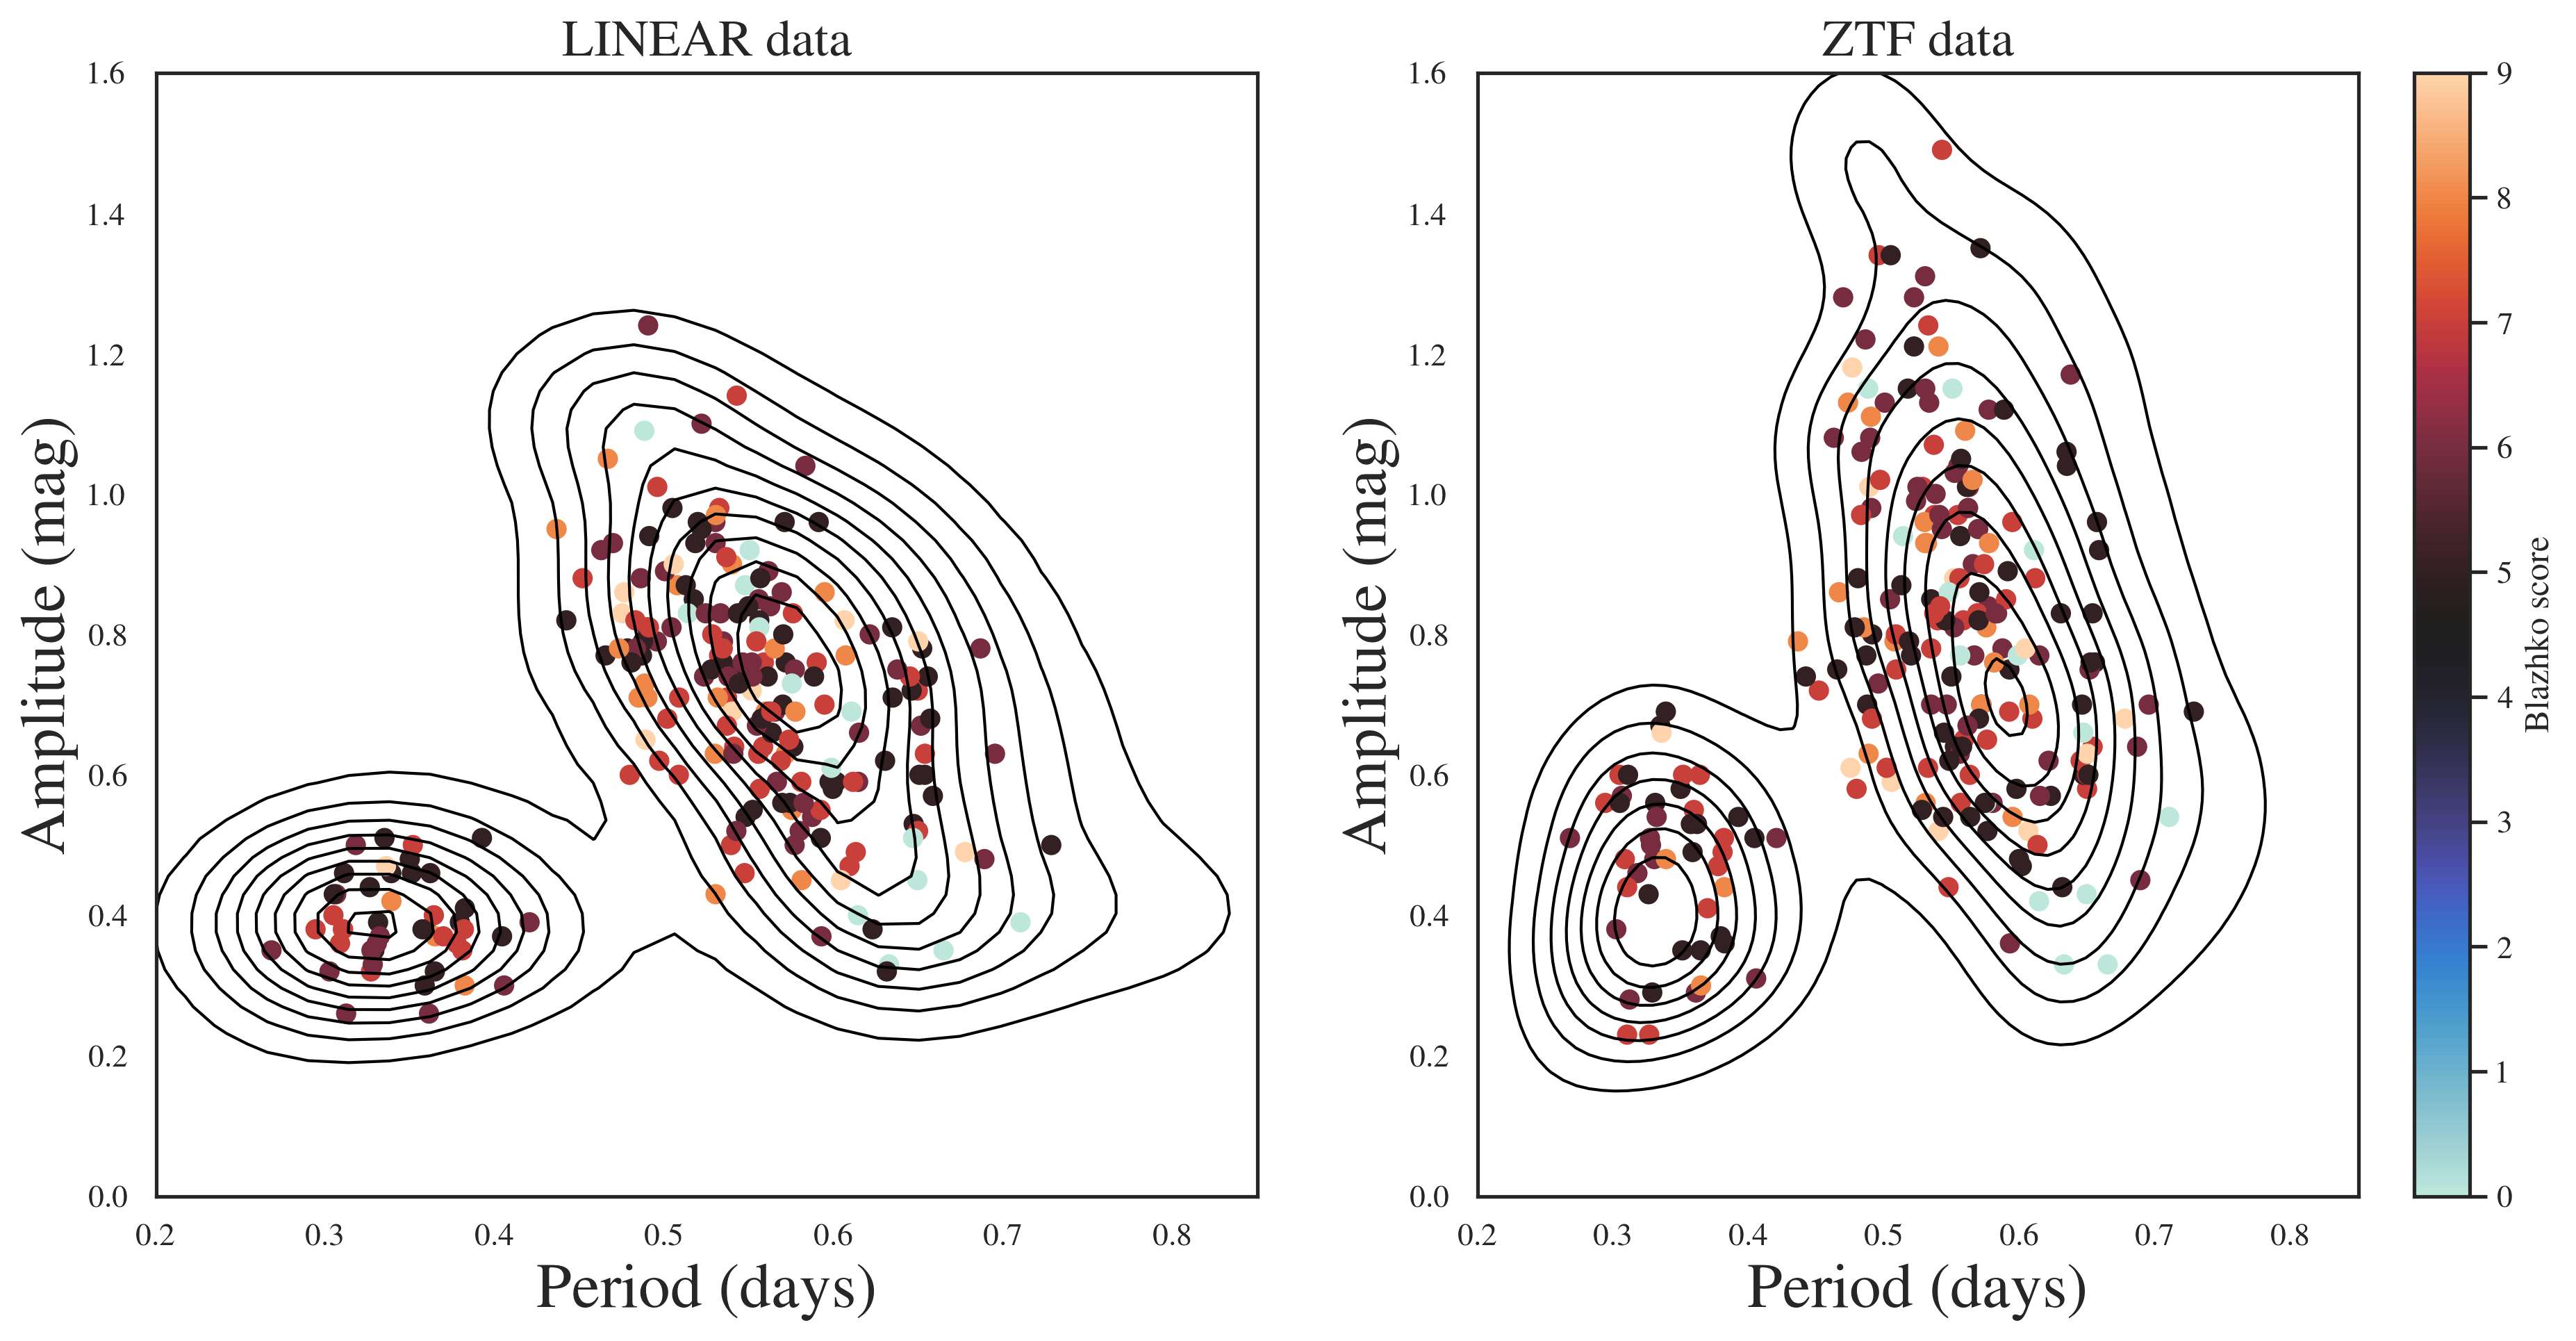
\includegraphics[width=16cm]{AmplPeriod.png}}
  \caption{Comparison of amplitude--period distributions (the Bailey
    diagram) for the starting sample of 1,996 RR Lyrae stars (contours)
      and 228 selected candidate Blazhko stars (symbols). The clump
      in the lower left corresponds to c type RR Lyrae and the
      other one to ab type. Note that the period distribution for ab
    type Blazhko stars is shifted left (by about 0.03 day, or 5\%).}
    \label{fig:AmplPeriod2D}
\end{figure*}


\begin{figure*}[ht]
  \centering
  \resizebox{\hsize}{!}{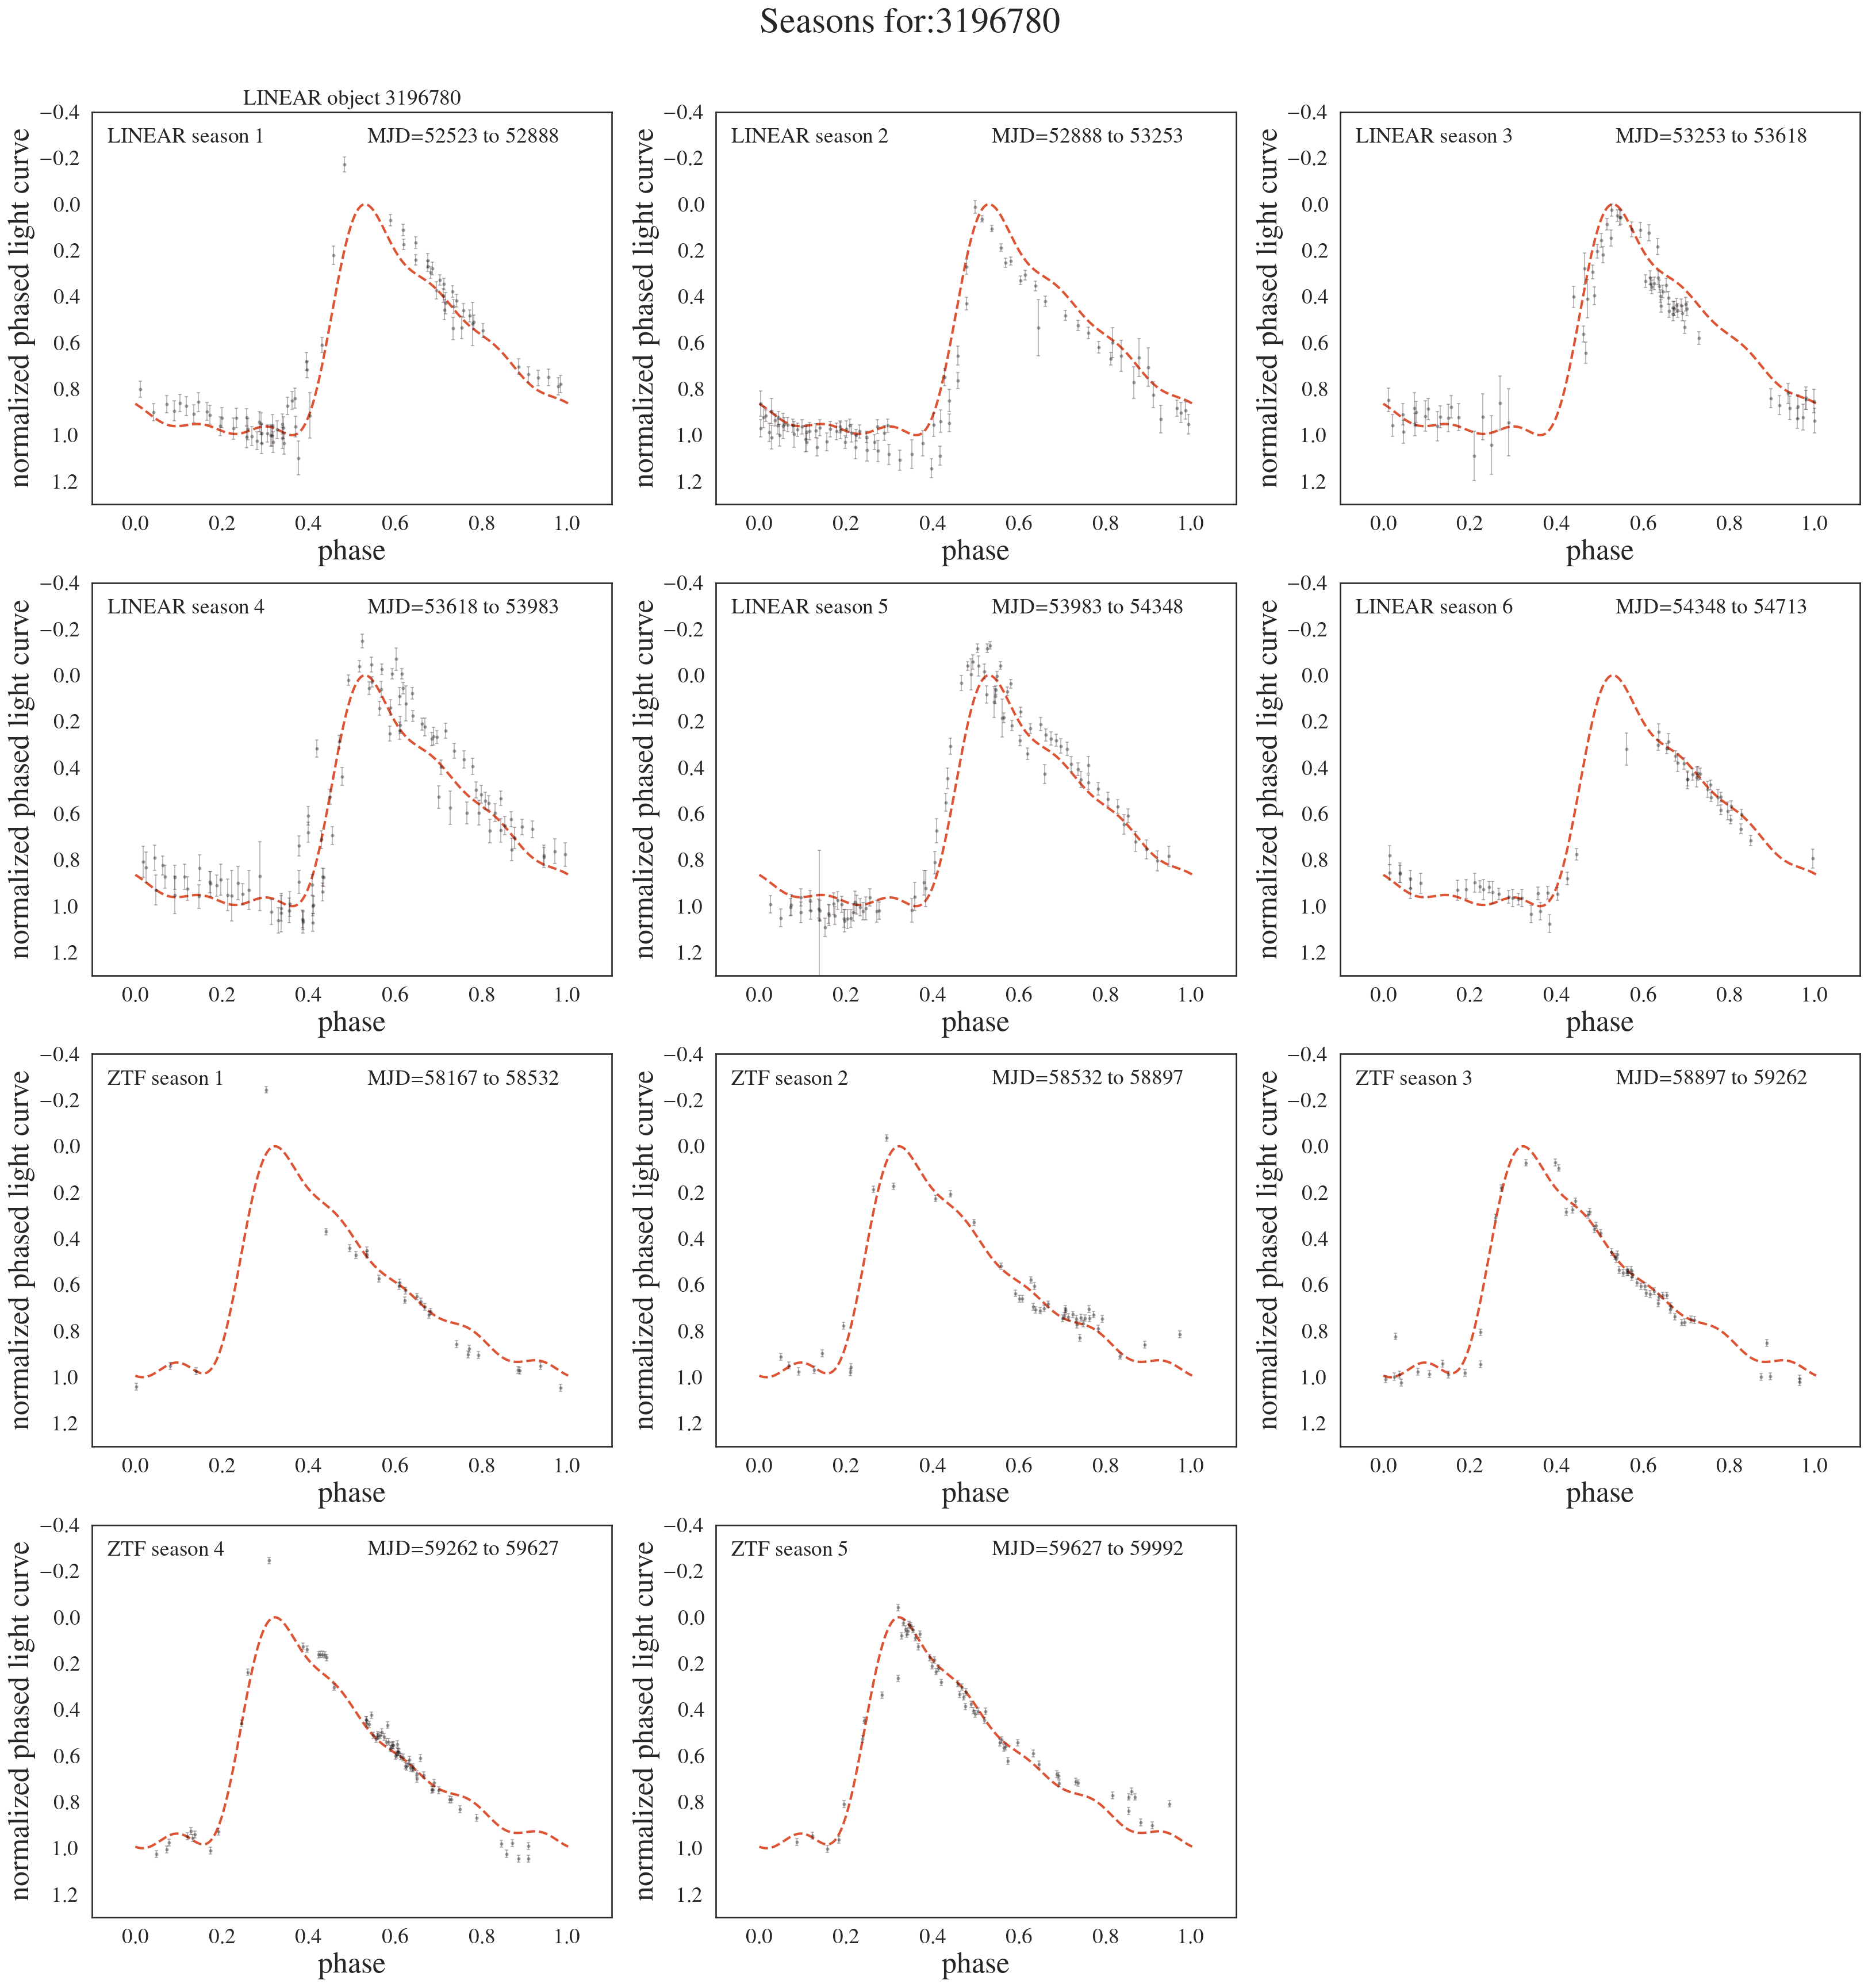
\includegraphics[width=16cm]{3196780_sn.png}}
  \caption{Analogous to Fig.~\ref{fig:phase4}, except that star
  with LINEARid = 3196780 is shown. Amplitude modulation is clearly
  seen in LINEAR light curves (top two rows), while not discernible
  in ZTF light curves (bottom two rows). Additional stars with
  similar behavior include LINEARid = 2889542, 7723614, 8342007.
  This behavior strongly  suggests that Blazhko effect can appear and disappear on time scales shorter than
    about a decade.
    }
    \label{fig:phase6}
\end{figure*}

Starting with a sample of 2857 field RR Lyrae stars with both LINEAR and ZTF data, we constructed a subsample of
1996 with light curves of sufficient quality and selected and verified 228 stars that exhibit convincing Blazhko effect.
In this section we compare various statistical properties of selected Blazhko stars to those of the starting sample. 

\subsection{The Blazhko Incidence Rate}

The implied incidence rate for the Blazhko effect is
11.4$\pm$0.8\%. Due to selection effects and unknown completeness,
this rate should be considered as a lower limit. 
When ab and c types are considered separately, the
rate is slightly higher for the former than for the latter: 12.1$\pm$0.9\%
vs. 9.2$\pm$1.3\%.  The difference of 2.9\% has low statistical significance ($<2\sigma$). 


\subsection{Period, Amplitude and Magnitude Distributions}

 
Marginal distributions of  period, amplitude and apparent magnitude
for the starting sample and Blazhko stars are compared in Fig.~\ref{fig:AmplPeriod}. 
Encouragingly, their magnitude distributions are statistically
indistinguishable which indicates that the completeness is not a
strong function of the photometric signal-to-noise ratio. This
result is probably due to the fact that the sample is defined by the
depth of LINEAR survey, while ZTF survey is deeper than this limit and
its photometric quality is approximately constant across the probed
magnitude range. 

The suspected differences in amplitude and period distributions are
further explored in Fig.~\ref{fig:AmplPeriod2D}. It is already
discernible by eye that the period distribution for Blazhko stars of
ab type is shifted to smaller values than for the starting sample. We have
found that the median period for ab type Blazhko stars is about 5\% shorter
than for the starting RR Lyrae sample. This difference is significant at
the 7.1$\sigma$ level.  At the same time, the difference in median
amplitudes for ab type stars corresponds to only 0.6$\sigma$ deviation. 
No statistically significant differences are found in period and
amplitude distributions for c type stars.

If modulation amplitudes are correlated with periods such that larger
modulation amplitudes occur in shorter period RRab stars, and if
our selection efficiency is lower for smaller modulation amplitudes,
then the detected period shift for ab type Blazhko stars might be at
least partially due to combination of these two effects. This
possibility does not appear likely. First, as we discussed in
preceeding section, our sample is defined by the depth of LINEAR survey, 
while ZTF survey is significantly deeper than this limit and its photometric quality is approximately constant across the probed 
magnitude range. Since it is sufficient for a star to display the
Blazhko effect only in ZTF to be included in the sample, 
we do not expect strong selection effects (except for the LINEAR
magnitude cutoff of course).  Furthermore, \cite{2020MNRAS.494.1237S}
searched for period - modulation amplitude correlation using a large
sample of stars with OGLE measurements and did not find any. 
 

\subsection{Long-term behavior of Blazhko Stars}

During visual analysis, we noticed that some Blazhko stars exhibit
convincing Blazhko effect either in LINEAR or in ZTF data, but not in
both surveys. Fig.~\ref{fig:phase6} shows an example where amplitude
modulation is clearly seen in LINEAR light curves, while not discernible
in ZTF light curves.  There are also examples of stars where Blazhko effect is evident in
ZTF but not in LINEAR data (e.g., LINEARid = 19466437, 14155360). 
This finding  strongly suggests that Blazhko effect can appear and disappear on time scales shorter than
about a decade.

 